
%\section{UI Gesture Collection} \label{section:UI_Gesture_Collection}
%
%In order to create a mapping from commands, as issued by the users, to a set of individual robot programs for multi-robot command and control, the gesture set for the commands must first be specified. 
%Multitouch gesture sets as a command language for controlling robots have been developed by an empirical process with naive users \citep{Micire:2009:ANG:1731903.1731912}. 
%These gestures frequently consisted of sequences of gestures that roughly fit the linguistic structure of a sentence, with the first gesture indicating the subject of the sentence, and the next gesture indicating a verb and possibly an object. 
%As a consequence, the gestures form a sort of language, and commands are sentences in the gesture language.
%A user might select a group of robots by circling them. 
%These robots would be the subject of the ``sentence''.
%Then the user might draw a path or tap a spot on a map, indicating that the robots should ``go here''. 
%Taken all together, the sentence could be read as ``these robots, follow this line to this location'', with the referents disambiguated by the locations of the command gesture on the screen.
%
%One way to define such an interface would be to select a fixed set of gestures, and then train the users to use those gestures when they interact with the system. 
%However, if the system is not one that the users use frequently, they will forget the training. 
%Since the advent of multitouch interfaces for smartphones and the trackpads of some laptops, many users already have some prior experience with multitouch gesture controls in everyday life. 
%Multitouch gestures can also be imitations of the way the users would expect to interact with material objects. 
%For example, zooming out of a map view by pinching two fingers together imitates the distant points of the map becoming closer together, indicating outward zoom, and spreading the fingers imitates stretching a smaller region to cover the screen for an inward zoom. 
%From these ``naturalistic'' expectations and daily use, users already have some idea of how a multitouch user interface can work. 
%If the interface fulfills the users' expectations, the users will find it easier to learn to use. 
%
%In other work, for each available command, one or two gestures were sufficient to cover the gestures used by 60\% or more of the users\citep{Micire:2009:ANG:1731903.1731912}. 
%However, it  is possible that there is no common gesture across users for a given task.
%If no two users use the same gesture for the same commands, or, more generally, there is very poor inter-user similarity for the gestures chosen to issue a command, then the approach of defining gestures from the user input does not offer useful guidance. 
%
%In order to determine if the chosen gestures change with the size of the swarm, tests will be conducted with varying swarm sizes performing the same tasks. 
%The swarm used for these tests will be large, with the lower bound on its size being significantly larger than the number of fingers a user could potentially gesture with. 
%In order to have a less tongue-in-cheek definition of ``large'', the scale required for a swarm to be considered ``large'' will be determined empirically.
%It is expected that there exists a transition point for the number of members in a swarm where users will stop interacting with the UI representation of the members of the swarm as individuals, and attempt to interact with the representations as groups or collections. 
%
%A large swarm is, then, a swarm with a number of members above the point at which such a transition occurs

\subsection{Introduction} \label{section:Introduction}

Multitouch gestural interfaces, like those found on tablets and smartphones, offer the possibility of a very direct user experience, especially compared to the Windows, Icons, Mouse, Pointer (WIMP) interface design. 
Rather than, for example, using an arrow key to scroll in a document, the user can drag the document directly, as though they were sliding a long piece of paper on a table. 

This directness is a hallmark of what has come to be called Natural User Interfaces, or NUI. 
A natural user interface is one that allows the user to re-use existing skills and natural motions to interact directly with content \citep{blakeNUIWin}. 
In practice, this means that the elements of the interaction are actions such as pointing and other gestures, drawing with a pen, speech, gaze, and so forth, rather than computer-specific interface devices. 
By way of contrast, the command line interface is defined in terms of typing with some form of keyboard, and the graphic user interface is (in most cases), defined in terms of mouse actions. 

However, as the number of operations the user wishes to perform increases, the limitations of multitouch screens become more apparent. 
Screens are flat, and so only afford 2-dimensional gestures, such as dragging, poking, and tapping. 
Even if the screen depicts a 2-dimensional projection of a 3-dimensional world, operations that would make sense in the 3D world, such as grasping, have to be mapped to the 2-dimensional space of operations to be performed. 
Typically, the gestures that the user uses to perform the available operations are chosen by the interface developer, and the user is trained to perform them, possibly by a short tutorial program \citep{wobbrock2009user, vanacken2008ghosts, freeman2009shadowguides}. 

Unfortunately, the use of screens with interactions inspired by the affordances of physical objects leads to the user having to decide between ``natural'' skills and motions, which are used on physical objects, and the skills and actions used with screens: single-point dragging and clicking. 
Most users understand that they are looking at pictures of things on a screen, and so default to single-point interactions \citep{vanacken2008ghosts}.
Further, tangible UIs, a subset of UIs that include real, physical objects for the user to interact with, raise a set of possible interactions that the designer may not forsee, or that the system may not be able to support \citep{hornecker2012beyond}.
Attempting to leverage the affordances of a physical object by depicting it on a screen adds another gap, where, in addition to failing to account for all of the affordances of the physical object (e.g. hitting it with another object), the system also fails to account for the affordances of a picture of an object (e.g. shrinking or enlarging it, which a real object cannot easily do). 
Additionally, even if these affordances are handled, they may not have clear meaning. 
What does it mean to use a photograph to hit a text file?

The behavior of users interacting with an NUI device is not solely informed by their intuitions about the physical objects represented on the screen. 
Smartphones, tablets, and other multitouch user interface devices, as well as specific types of computer programs, such as CAD and realtime strategy game programs, also inform the user's expectations about interactions with new interfaces. 
Rather than claiming that the users are untrained, and the gestures are ``intuitive'', it would be more accurate to claim that the users already have a form of training, from the devices that they use in their daily lives. 
We attempt to discover the gestures that users would choose themselves, based on their own thinking about the interface and their own past experience with computer technology such as tablets, smartphones, and video games. 

User-defined gestures have advantages in memorability and user preference over gestures designed by the researcher or interface programmer \citep{nacenta2013memorability}. 
However, the study that indicated this preference was for gestures that each user defined for themselves, rather than a gesture set that was constructed by eliciting gestures from the users and compiling a gesture set as in \citep{Micire:2009:ANG:1731903.1731912}. 

This work is an extension of previous work that used a similar process to discover user interface gestures for single or small groups of robots \citep{Micire:2009:ANG:1731903.1731912}. We extend this method from groups to larger swarms of robots, in an attempt to discover if the gestures that users select vary with the number of robots available.

More specifically, it is hypothesized that there exists a swarm size beyond which users will transition from treating the swarm robots as individuals to interacting with the robots in small groups or as a single large group. 
This transition point will be apparent because of a change in the gesture set that users choose to interact with the swarm. 
Rather than issuing one command for each robot, the user will instead use commands that control the bulk of the robots as a cloud or flock, but may leave some robots unused. 
For example, the user may switch from selecting robots as individuals to shaping the group as if sculpting, with pushing and pinching to ``carry'' groups around. 
The user may also change how they indicate which robots are to be interacted with. 
Rather than selecting each robot by clicking on it, the user might circle a group they want to use, or simply assume that the same command is issued to all robots by default. 
The size of the swarm where changes in the user gestures occur will indicate the transition point between the user intending to interact with individual robots as opposed to interacting with the swarm as a whole. 

Further, it is hypothesized that altering how the user interface displays the location of the robots in the swarm will affect the transition point.
Once the ratio of the size of individual swarm members to the size of the area the swarm is in becomes sufficiently small, displaying the swarm members at the same scale as the map will result in the representation of the swarm members being too small to interact with. 
Scaling the representation of the robots up, relative to the map, could make the robot representations overlap unrealistically and obscure the map. 
Instead, we propose that for certain scales of swarms, it makes sense to represent the swarm as the area covered by the swarm, rather than the locations of the individual robots.
This approach has been used successfully for navigation in three dimensions, by developing a controller that causes the individual UAVs to remain within a bounding prism, and allowing the user to control the shape and location of that prism, instead of the location of each individual UAV \citep{ayanian2014controlling}.
 
More specifically, a display which obscures individual robots and displays a cloud or swarm boundary will cause the user to treat the swarm as a whole rather than individuals, which will be apparent because the user will use the same gestures that users select for controlling individual robots. 

\subsection{Experiment Setup} \label{section:Experiment_Setup}

Users were seated in front of the interface and read a script describing the system and the experiment. The user interface displayed alternating slides of instructions to the user, such as ``Move the robots to area A", and interface screens for them to interact with. 
The interface did not visibly respond to user contact or move the robots depicted on it.
In this regard, it more closely resembles the paper prototypes of the User-Centered Design process than a fully functional interface \citep{ehn1992cardboard}.

The multitouch user interface device used in this experiment is a 3M M2265PW touchscreen. 
This screen can track up to 20 simultaneous points, but reports only points, rather than shapes or areas of contact. 
While the user interacted with the touch screen, their touches and the positions of their hands were recorded by the computer connected to the screen and by the video cameras. 
One video camera was placed high, looking down at the screen, to track where the user's hand position over the screen. 
The other video camera was placed in front of the screen at a low angle, in order to observe whether the user's hands were touching the screen, or moving above it. 
In addition to screen contacts and video, users were asked to think aloud about their actions.
A microphone placed near the screen was used to record everything the user said. 

\begin{figure}
	\centering
	\includegraphics[width=\linewidth]{/home/ams/TinyRobo/docs/setup.png}
	\caption{Experiment setup, showing, L to R, the survey computer, microphone, cameras and multitouch interface device, and an example robot.}
	\label{fig:experiment_setup}
\end{figure}

The software used to record all of this information is ROS, the Robot Operating System \citep{ROS_announcement_paper}. 
ROS was developed as a message-passing framework and hardware abstraction layer for robots. 
Software using ROS is implemented as ``nodes'', which communicate by passing messages, generally in a publisher/subscriber pattern. 
The format of the messages is formally defined, and the generation of the code for generating messages and handling routing of messages is provided by ROS. 

It may seem unusual to use a framework intended for operating robots as a recording program for collecting experiment data, but ROS provides a utility called rosbag that records some or all of the messages emitted by the robot's sensors in a ``bag'' file. 
In this case, the cameras, microphone, and UI application are the ``sensors'' which rosbag records.
A ROS launch file starts multiple ROS nodes to record image data from the cameras, audio from the microphone, and touch events and screen updates from the UI.
ROS also provides tools for manipulating bag files, and playing them back. 
All of the data in the file is timestamped, so it plays back with the audio, video, and UI interactions all accurately synchronized. 
Because all of the data is treated as standard ROS message types, it is relatively easy to write custom processors for the recorded data.
For example, a node was written that accepts the replayed UI screen changes and touch events, and renders them as a stream of ROS image messages showing the contact points overlaid on the UI screen. 
Ultimately, the entire data stream was rendered to video, as the rosbag playback does not support rewinding the playback, and being able to re-view a section conveniently was useful for coding. 

\subsubsection{Experiment Conditions} \label{section:Experiment_Conditions}

Each user was assigned to one of five conditions, varying by how many robots were in each condition. 
The conditions consisted of 1-2 robots, 10 robots, 100 robots, 1000 robots, or an unknown number of robots.
In the unknown number condition, the area the robots were present in was represented by a cloud. 
For each condition, the user was requested to perform a sequence of tasks. 
The exact number of tasks varied between conditions due to some tasks not making sense with the number of robots involved. 

\begin{figure}
	\centering
	\begin{subfigure}{0.4\textwidth}
		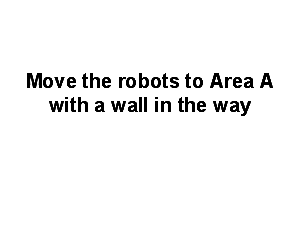
\includegraphics[width=\linewidth]{../ui_experiment/slide_images/Swarm_Robot_Control_-_10_Robot_0004.png}
	\end{subfigure}
	\begin{subfigure}{0.4\textwidth}
		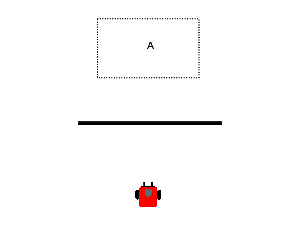
\includegraphics[width=\linewidth]{../ui_experiment/slide_images/Swarm_Robot_Control_-_Single_Robot_0005.png}
	\end{subfigure}
	\begin{subfigure}{0.4\textwidth}
		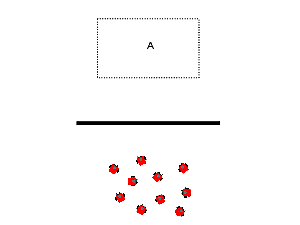
\includegraphics[width=\linewidth]{../ui_experiment/slide_images/Swarm_Robot_Control_-_10_Robot_0005.png}
	\end{subfigure}
	\begin{subfigure}{0.4\textwidth}
		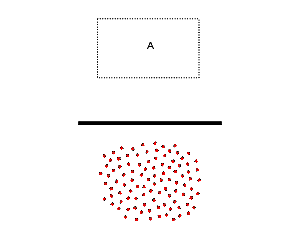
\includegraphics[width=\linewidth]{../ui_experiment/slide_images/Swarm_Robot_Control_-_100_Robot_0005.png}
	\end{subfigure}
	\begin{subfigure}{0.4\textwidth}
		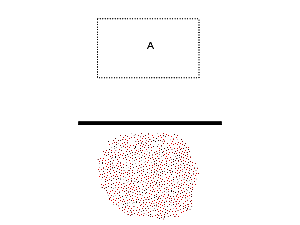
\includegraphics[width=\linewidth]{../ui_experiment/slide_images/Swarm_Robot_Control_-_1000_Robot_0005.png}
	\end{subfigure}
	\begin{subfigure}{0.4\textwidth}
		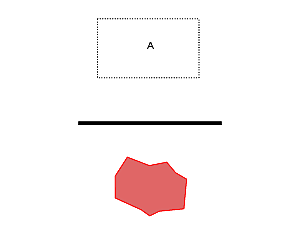
\includegraphics[width=\linewidth]{../ui_experiment/slide_images/Swarm_Robot_Control_-_Unknown_Number_of_Robots_0007.png}
	\end{subfigure}
	\caption{Instructional slide and situations for moving around the wall to area A, in each condition.}
	\label{fig:move_around_wall}
\end{figure}

\begin{tabular}{l|l|l|l|l|l}
& 1 & 10 & 100 & 1000 & Unknown \\
Move to area A & x & x & x & x & x\\
Move to area A with a wall & x & x & x & x & x \\
Stop the robots & x & x & x & x & x\\
Divide around an obstacle & & x & x & x & x \\
Orange to B, red to A & x & x & x & x & x \\
Orange to A, red to B & x & x & x & x & x \\
Orange to A, red to B (mixed) & x & x & x & x & x \\
Divide group & x & x & x & x & x \\
Merge groups & & x & x & x & x \\
Form a line & & x & x & x & x \\
Form a square & & x & x & x & x \\
Move the crate to area A & x & x & x & x & x \\
Move the crate to area A (dispersed) & x & x & x & x & x\\
Mark defective robot & x & x & x & x & \\
Remove defective robot & x & x & x & x &  \\
Patrol the screen border & x & x & x & x & x \\
Patrol area A & x & x & x & x & x \\
Disperse over screen & x & x & x & x & x \\
\end{tabular}

The individual robot case is lacking the tasks that do not make sense for a single robot. A single robot cannot, for example, divide around an obstacle or form a square. 
The ``Merge groups" task was left out of the single robot case because of the potential for confusion when referring to a single robot as a group. 

The unknown number of robots condition has the same tasks as the 10, 100, and 1000 robot cases, except for the ``Mark defective robot" and ``Remove defective robot" task. 
Without UI elements that represent individual robots, the user cannot take any actions that refer to a specific robot. 

\subsection{Analysis} \label{section:Analysis}

User gestures were coded using a methodology adopted from the social sciences, Grounded Theory \citep{glaser2017discovery}.
Grounded Theory is an iterative process, where the data are first coded at a very fine-grained level, and then the resulting coded elements are compared to each other to try to determine their qualities, similarities, and differences. 
Codes can be consolidated or divided until repeated passes of coding and comparison no longer alter the emerging structure of the coding scheme. 
During each iteration of coding and comparison, the coder makes memos as well, describing the links they see between related coded elements and higher-level abstractions that relate the elements. 
These memos are eventually written up as the social scientific theory, which is believed to be grounded in the data because it arises from the coding process. 

\subsubsection{Initial coding pass} \label{section:Initial_coding_pass}

The inital pass used open coding, where the ``codes'' were essentially free-form text entry. 
Rough counts of the open codes for the first 10 participants indicated that ten of the codes covered 81\% of the 580 total coded events. 
The ten most heavily used codes are, in order of occurrence: drag, tap, voice command, box select, 2 finger drag, double-tap, lasso, tap and hold, 2 handed drag, reverse pinch, and parallel hands. 
This pass of coding indicated that a majority of the user actions could be coded as some form of drag, some form of tap, box or lasso selection, pinch, and parallel hands. 
The final gesture, ``parallel hands'' is placement of the hands, palms facing each other, over some area of the screen. This gesture was used many times by the same user who issued voice commands, to indicate where the robots should form a line. Because parallel hands only accounted for 0.69\% of the gestures, it was left out of the development of the coding application for the second stage of coding. 

The most common code was drag, which accounts for 37.58\% of the rough coding, or 42.07\% if all forms of drag in the top ten codes are considered. ``Drag'' is when the user places one finger down, moves it to another location, and raises it again. Two finger drag is the same, only with two fingers on the same hand placed on the screen rather than one. Two-handed drag is single-finger drag, but executed with both hands at the same time. 

The second most common code was ``tap'', with 20.34\% of the rough coding, or 25.34\% if tap, double-tap, and tap and hold are all considered. Tap is when the user places a finger down and then very quickly raises it again. Double-tap is two taps in the same location in quick succession. Tap and hold is when the user places their finger on the screen and leaves it in one place for more than a second before raising it. 

Box select consists of a diagonal (relative to the screen edges) drag gesture over the robots or another object on screen, with the intent to select everything within the box whose diagonal is represented by the drag. 
Lasso select is a drag which ends near where it began, forming a loop, with the intent to select everything inside the loop. 

Pinch and reverse pinch are essentially two-hand drag or two-fingered drag but with the hands or fingers moving towards (pinch) or away (reverse pinch) from each other.
This gesture is common for zooming in multitouch user interfaces on smartphones. 

Voice command was used to code when a user spoke a command out loud, rather than using gestures. The high incidence of voice commands (7.07\% of all codes) in the first ten users can be attributed to a single user who issued commands almost exclusively through voice. 
 
\subsubsection{Second Coding Pass} \label{section:Second_Coding_Pass}

To facilitate coding in the second pass, an application was developed to record codes. 
The application has coding functions for the six most common gestures: drag, tap, voice command, box select, lasso select, and pinch. 
It also includes coding functions for user interface elements described by the user, such as buttons or menus, a function to code user gestures not covered by the six most common gestures, and a function for coders to enter free-form text memos. 

\todo{Need to make the call as to whether example gestures that users made should be counted along with ``real'' gestures, or left out. Maybe go both ways and see if it affects anything.}

A second pass of coding of the first ten user recordings was performed by two coders. 
Because the coders were responsible for deciding which user actions to code, as well as how to code them, it is possible for one coder to miss a gesture that another coder codes, or to split a single gesture into two coded units instead of one. 
For example, one coder initially split spoken commands at conjunctions such as "and", resulting in two units both coded as voice commands, while the other coder coded the entire sentence as a single unit. 
This leads to the possibility that for a single task, the coders will produce different length lists of coded units. 

Cohen's $\kappa$ is a measure of inter-coder reliability for categorical items, but it assumes that both coders are coding the same number of codable units \citep{cohen1960coefficient}. 
In order to calculate inter-coder reliability in the presence of potentially missing data, the  shorter of the two lists of codes for each task padded with a code for ``no data". 
The codes were then aligned chronologically, with pair consisting of an item from each list such that the total time error within the task was minimized.
As a result, the alignment process created pairs of a valid code and the ``no data" code for the codes in the longer list that did not have a good chronological match in the shorter list.
This was based on the assumption that the source of the error is one coder missing an event that did occur, rather than the other coder coding an event that did not occur. 

The initial pass of coding got poor inter-coder reliability, with the first 10 participants having Cohen's $\kappa$ of 0.357, 0.266, 0.398, 0.387, 0.643, 0.428, 0.407, 0.56, 0.273, and 0.502. 
Cohen's $\kappa$ of over 0.75 is excellent agreement, 0.4-0.75 is fair, and below 0.4 is poor, so the average $\kappa$ was barely above the cutoff for fair agreement. 

Analysis of the data, particularly with confusion matrices, showed several problems. 
The simplest was training error in the training of the coders.
One coder had not been instructed that the ``UI'' code existed, and so had coded user interface widgets as ``tap'' events.   
This was immediately apparent in the confusion matrix as a very high confusion between ui and tap events. 
The other main source of confusion was lasso and box selection actions being coded as drag events, and vice versa.
The actual action performed in a lasso is a drag, in that the user puts their finger down and drags it in a circle around something before lifting it again, but it is intended as a selection of the things inside the circle rather than e.g. drawing a circle shape. 

In order to reduce these errors, and ensure consistency in training the coders, the descriptions for each code were written up in discussion with the coder, so that questions about interpretations could be answered in advance and recorded. 
Another coder was trained with the code description document, and coded the first 5 participants. 
This coder obtained Cohen's $\kappa$ of 0.728, 0.927, 0.75, 0.827, and 0.738 with one of the original coders.
These values indicate a very high level of agreement, so the remaining videos were coded by these two coders, using the description of the codes from the code description document.  

The resulting data set has 3,256 individual gestures coded. 
In coding, the codes were box selection, lasso selection, drag, tap, pinch, ui widgets, voice command, and other. 
\todo{Insert text of coding document}
For analysis, drags that were used to draw something on the screen were separated from non-drawing drags. 
Taps were separated into single, double, and triple taps, plus tap and hold. 
Pinch was separated into pinch (where the contact points move towards each other) and reverse pinch (where the contact points move apart).
All of these divisions were based on modification flags used during the coding process.  

\begin{tabular}{l r r}
gesture & count & percent\\
drag & 1084 & 33.2924 \\
draw & 761 & 23.3722 \\
tap & 514 & 15.7862\\
other & 189 & 5.8047 \\
lasso & 184 & 5.6511 \\
box & 113 & 3.4705 \\
ui & 112 & 3.4398\\
double tap & 95 & 2.9177 \\
hold & 66 & 2.0270\\
reverse pinch & 49 & 1.5049 \\
voice & 44 & 1.3513\\
pinch & 26 & 0.7985 \\
triple tap & 19 & 0.5835\\
\end{tabular}
\todo{Add caption, label. Also, this includes examples, maybe break out non-examples so the totals match total counts in later sections.}

\section{Selection Gestures} \label{section:Selection_Gestures}
One area in which the gestures were expected to change between conditions is the use of selection gestures. 
The intuition behind this expectation is that for small numbers of robots, there is no need for a gesture that selects groups, as the user can interact directly with each robot. 
Similarly, in the case where no individual robots are displayed, the use of group selection gestures would be minimal, as the group is presented as a single cloud. 

Users performed selection of robots in groups by box select, lasso, and UI interactions.
These selections were counted by condition by counting lasso or box events that had a robot or robots as their targets. \todo{The std dev for a lot of these is bigger than the data, very high variability. Discard outliers? There are only ten users per condition to begin with}
 
\begin{table}
	\centering
	\begin{tabular}{l r r r r}
		Condition & Box Select & Lasso & Tap & Total (condition)\\
		\hline
		unknown & 0 & 1 & 43 & 44 \\
		one & 0 & 3 & 78 & 81\\
		ten & 26 & 105 & 140 & 271\\
		hundred & 68 & 53 & 35 & 156\\
		thousand & 18 & 16 & 22 & 56\\
		\hline
		TOTAL & 112 & 178 & 318 & 608\\
	\end{tabular}
	\caption{Per-condition total use of selections}
\end{table}

Single selections of robots were performed by tapping on the robot. 
Similarly to the count of group selections, tap events were counted where the object of the tap event was a robot or robots. 

The ten robot case has the most selection gestures for either group or single selection. 
As was expected, the unknown number and single robot cases have very low counts of group selections. 
Interestingly, the thousand robot case also has relatively low group and single 
selection use, especially compared to the ten robot case. 

To determine if these differences were statistically significant, the count of each user's gestures per task were normalized by dividing by the total number of gestures that that user used to perform the task. 
Normalizing in this manner converts raw gesture counts to a proportion of the total gestures used on that task, which prevents more verbose users from dominating the analysis.

The tasks checked for statistically significant differences between conditions were those that all conditions had in common. 
These nine common tasks are `move crate', `divide by color (cross)', `divide by color', `move to a', `move to a (wall)', `patrol a', `patrol screen', `split', and `stop'. 
Across all the common tasks the proportions of each gesture were collected per gesture, resulting in, for each gesture, 5 lists, one for each condition. Each list consists of 90 entries, 10 users times 9 common tasks. Each list entry consists of the proportion of that gesture the user used to complete the task. ANOVAs were performed for each pair of conditions. 

% This is PER-USER normalization, but PER TASK normalization is what I want
%For uses of tap as selection across the common tasks, the unknown number condition differs from the hundred (F=8.8744, p=0.0033) and thousand (F=4.8577, p=0.0288) robot conditions. 
%The one robot condition differs from the ten (F=4.5036 , p=0.0352), hundred (F=13.7996 , p=0.0003) ), and thousand (F=10.4596, p=0.0014) robot conditions.
%The ten robot condition differs from the hundred robot condition (F=4.2012, p=0.0419).
%These differences are summarized in table \ref{tab:tap_select_per_user_norm}.
%
%\begin{table}
%	\begin{tabular}{l|l l l l l}
%		& unknown & one    & ten        & hundred     & thousand   \\ 
%		\hline
%		unknown & & 0.1066 & 0.4915 & \textbf{0.0033} & \textbf{0.0288} \\   
%		one & & & \textbf{0.0352} & \textbf{0.0003} & \textbf{0.0014} \\
%		ten & & & & \textbf{0.0419} & 0.1828   \\
%		hundred & & & & & 0.3132   \\
%		thousand & & & & &\\
%	\end{tabular}
%	\caption{p-values for the use of tap as select between conditions}
%	\label{tab:tap_select_per_user_norm}
%\end{table}

For uses of tap as selection across the common tasks, the unknown number condition differs from the hundred (F=7.6964, p=0.0061) and thousand (F=5.5772, p=0.0193) robot conditions. 
The one robot condition differs from the ten (F=4.3299, p=0.0389), hundred (F=13.5889, p=0.0003), and thousand (F=10.4274, p=0.0015) robot conditions.
These differences are summarized in table \ref{tab:tap_select_per_user_norm}.

\begin{table}
	\begin{tabular}{l|l l l l l}
		& unknown & one    & ten        & hundred     & thousand   \\ 
		\hline
		unknown & & 0.5622 & 0.1772 & \textbf{0.0006} & \textbf{0.0193} \\   
		one & & & \textbf{0.0389} & \textbf{0.0030} & \textbf{0.0015} \\
		ten & & & & 0.1089 & 0.2719   \\
		hundred & & & & & 0.5457   \\
		thousand & & & & &\\
	\end{tabular}
	\caption{P-values for the use of tap as select between conditions}
	\label{tab:tap_select_per_task_norm}
\end{table}

For uses of group selection across the common tasks, the unknown number condition differs from the ten (F=47.635915, p<0.0001), hundred (F=60.435124, p<0.0001) and thousand (F=10.2346959, p=0.0016) robot conditions. 
The one robot condition differs from the ten (F=47.6359, p<0.0001), hundred (F=60.4351, p<0.0001), and thousand (F=10.2347, p=0.0016) robot conditions.
The ten robot condition differs from the thousand robot condition (F=19.0110, p<0.0001).
The hundred robot condition differs from the thousand robot condition (F=30.2373, p<0.0001).
The identical F and p values for the one and unknown robot conditions and the various conditions that they differ from are because for the one and unknown robot conditions, no group selection gestures were used in the common tasks. 
These differences are summarized in table \ref{tab:group_select_per_task_norm}.

\begin{table}
	\begin{tabular}{l|l l l l l}
		& unknown & one    & ten        & hundred     & thousand   \\ 
		\hline
		unknown & & * & \textbf{0.0000} & \textbf{0.0000} & \textbf{0.0016} \\   
		one & & & \textbf{0.0000} & \textbf{0.0000} & \textbf{0.0016} \\
		ten & & & & 0.1808 & \textbf{0.0000}   \\
		hundred & & & & & \textbf{0.0000}   \\
		thousand & & & & &\\
	\end{tabular}
	\caption{P-values for the use of group selections between conditions. The ANOVA between the unknown case and the single robot case was not computable, as no group selections were used for the unknown case or the single robot case for the common tasks.}
	\label{tab:group_select_per_task_norm}
\end{table}

\begin{table}
	\begin{tabular}{l | l l}
		& common tasks & all tasks\\
		\hline
		unknown & 0 & 1\\
		one & 0 & 3\\
		ten & 55 & 107 \\
		hundred & 60 & 109\\
		thousand & 15 & 28\\
	\end{tabular}
	\caption{Counts of group selection gestures in the common tasks and all tasks.}
	\label{tab:group_raw_counts}
\end{table}

\begin{table}
	\begin{tabular}{l | l l}
		& common tasks & all tasks\\
		\hline
		unknown & 15 & 29\\
		one & 38 & 53 \\
		ten & 45 & 108\\
		hundred & 4 & 29 \\
		thousand & 7 & 18\\
	\end{tabular}
	\caption{Counts of tap selection gestures in the common tasks and all tasks.}
	\label{tab:tap_raw_counts}
\end{table}

Examining the non-normalized counts of taps as selections and group selections across both the common tasks and all tasks indicates that heaviest use of tap selection is in the ten robot case. Heaviest use of group selection is in the hundred robot case, but the ten robot case only lags it by two uses. The second heaviest for group selection is the hundred robot case, while the second heaviest for tap selection is the single robot case. This seems to indicate that with single robots, users prefer tap selection, with one hundred robots they prefer group selection, but with ten robots, either selection method could be viewed as appropriate. 

It was surmised that users may have been performing multiple tap selections in a row to select robots in the ten robot case, but that a 10-robot tap selection would be condensed by the normalization into the same proportion of the overall gestures as a single-robot tap selection. 
To check if users were performing multiple taps in a row as selections, the lengths of sequences of tap actions were checked across all cases. 
As seen in table \ref{tab:tap_seq_len}, while the ten robot case does have a much higher count of sequences of taps, the mean is higher than the other cases, and the standard deviation much higher. 
On examining the data, there was exactly one case of a 10-tap sequence in the ten robot case.
While it is possible that a user in the ten-robot case might perform a selection by tapping each of the ten robots, but it is not a common occurrence. 

\begin{table}
	\begin{tabular}{l | l l l}
		& Sequence Count & Mean Length & Standard Deviation \\ 
		\hline
		unknown & 28 & 1.0357 & 0.1856 \\
		one & 42 & 1.2619 & 0.5798\\
		ten & 72 & 1.5000 & 1.6499\\
		hundred & 23 & 1.2609 & 0.4391\\
		thousand & 17 & 1.0588 & 0.2353\\
	\end{tabular}
	\caption{Lengths of sequences of taps within conditions.}
	\label{tab:tap_seq_len}
\end{table}

% TRIPLE CHECK THIS BEFORE USING ANY OF IT
%For the box selection gesture, the unknown condition differs significantly ($\alpha$ = 0.05) from the ten (F=7.17386 p=0.00809), hundred (F=26.95175 P=0.00000), and thousand (F=4.57743 p=0.03376) robot conditions, but not from the single robot condition (F and p values could not be calculated due to disuse of box selection in these cases). 
%The use of box select in the one robot condition differs significantly from the ten (F=7.17386 p=0.00809), hundred (F=26.95175 p=0.00000), and thousand (F=4.57743 p=0.03376) robot conditions.
%The hundred robot condition differed from the ten (F=9.17884 P=0.00281) and thousand (F=13.81053 P=0.00027) robot cases. 
%
%
%
%For the lasso gesture, the unknown condition differs significantly from the ten (F=33.27742 P=0.00000), hundred (F=19.44664 P=0.00002), and thousand (F=5.86234 P=0.01647) robot cases. 
%The one robot condition differs significantly from the ten (F=33.27742 P=0.00000), hundred (F=19.44664 P=0.00002), and thousand (F=5.86234 P=0.01647) robot cases as well. \todo{Why are these differing by the same amount between unknown and one? The same proportions?}
%The thousand robot condition also differed from the ten (F=23.51414 P=0.00000) and hundred (F=11.76321 P=0.00075) robot conditions. 
%
%For the tap gesture, the unknown condition differs significantly from the one (F=5.07967 P=0.02543) and thousand (F=5.31693 P=0.02227) robot conditions. 
%The one robot condition differs from the ten (F=5.58672 P=0.01918), hundred (F=7.47952 P=0.00687), and thousand (F=21.15146 P=0.00001) robot conditions. 
%The thousand robot also differs from the hundred robot condition (F=4.08954 P=0.04465), although not as strongly as many of the others. 
%However, this analysis looks at all uses of tap, not just tap intended as select, as detected by the object of the tap being a robot.
%
%To determine if tap-as-select, rather than just any use of tap, maintained this relationship, the count of group selects (box or lasso with robots as the object) and single selects (taps with robots as the object), were collected, per user across all tasks that are common to all conditions. 
%These lists were averaged, to get the average use of group select or single select, for each task, averaged across the condition.\todo{This is raw counts, should maybe do this and then normalize to get proportions, rather than average.}
% 
%For tap-as-select, the hundred robot case differed from the unknown (F=5.61783, p=0.03068), one (F=9.13207, p=0.00810) , and ten (F=6.59643, p=0.02062) robot cases. The thousand robot case differed from the ten (F=5.64536, p=0.03033) and one (F=7.62757, p=0.013893) robot cases.
%
%For group select, the hundred robot case differed from the unknown (F=5.61783, p=0.03068), one (F=9.13207, p=0.0081) , and ten (F=6.59643, p=0.02062) robot cases. The thousand robot case differed from the ten (F=5.64536, p=0.03033) and one (F=7.62757, p=0.01389) robot cases.



%The gestures draw, pinch/reverse pinch, and double-/triple-tap did not display any statistically significant difference across conditions in the common tasks. 
%Pinch/reverse pinch were somewhat task-specific gestures, used across condition to divide/merge groups of robots in that task. 
%
%Draw is also somewhat task specific, mostly used in formations to draw the target shape. However, the formation tasks are not in the common task set, because a single robot cannot form a formation. 
%
%Were double and triple taps also specific to some task? This would be interesting to check, because it seems to indicate a division of gestures into gestures that were related to a task, and gestures that were related to a condition. 
%
%Graphing \todo{put the graphs in here} average per-user proportion of gestures per task indicates that pinch or reverse pinch were highest in divide color 1, patrol a, patrol screen, and split. Split had by far the most reverse-pinch gestures. 
%
%Draw peaked for split and stop. For split, this was caused by users drawing a dividing line between the split groups. For stop, it was caused by users drawing a line in front of the robots to indicate a virtual barrier. If the formation tasks were in the common task set, they would also likely have large numbers of draw gestures. 
%
%Doubletap peaked in the stop case as well, but triple taps occured at a very low level in crate, divide color 1, and move a, and at a slightly higher level in patrol screen and split. In general, tripletap may not have enough samples to make a comparison meaningful. It was only used 19 times total, and is the least common gesture. 

[DATA INTENSIFIES]

\section{Multi-hand Gestures}

Multi-hand gestures fall into two different groups. \
The first group is gestures where each hand is performing part of a single gesture.
Generally, these were pinches and reverse pinches with one finger on each hand. 
%[PUT COUNT HERE] users also performed two-handed drags with one finger of each hand. 
The other group of multi-hand gestures consists of a simultaneous pair of different gestures, one performed with each hand. 
For purposes of coding, dragging one object to one place with two fingers was coded as a single drag with two fingers, while dragging two objects to two different places was coded as two single-fingered drags at the same time. 

Fifty percent of the users performed at least one two-handed gesture. 
This is fewer than in some previous research, but more than might be expected if users were generalizing from single-point mouse interaction \cite{micire2010multi, epps2006study}
Epps et al required users to use a single hand for over half of the gestures in their study, and they point out that their use of a Windows desktop as the working environment of the study may have influenced people towards a single-point interaction style. 

There were 82 instances of two-handed gesturing. 
If this total is treated as 164 gestures, one for each hand, two-handed interactions account for 5.037\% of the gestures used.

\begin{table}
	\centering
	\begin{tabular}{l l}
		Gesture Pair & Count\\
		\hline
		drag and drag (different objects) & 26 \\
		pinch & 22\\
		reverse pinch & 7\\
		tap and tap & 6\\
		drag and tap & 6\\
		drag (same objects) & 5\\
		other and other & 5\\		
		box select and box select & 3\\
		box select and tap & 1\\
		box select and UI & 1\\
		\hline
		TOTAL & 82\\
	\end{tabular}
	\caption{Two handed gesture pairs. Note that the total is lower than the actual count of total gestures, since it counts e.g. two simultaneous drag actions as a single two-handed drag action.}
\end{table}

Most of the two-handed gestures were simultaneous drags of two different objects. 
Simultaneous drags and two handed pinches or reverse pinches account for 58.537\% of the two-handed gestures.  

Due to the prevalence of smartphone adoption, it is no longer simple to determine if smartphone use contributes to the use of pinch and reverse pinch gestures, because there are almost no smartphone non-users in the population of this study. 
Out of 50 subjects, 46 (92\%) reported using an Android or Iphone smartphone daily. 
Only one user did not report having used an Android or Iphone at least moderately, and stated that they did not own any touchscreen devices. 
Despite not having any touchscreens, even this user made two-handed gestures. 

\begin{table}
	\centering
	\begin{tabular}{l l}
		Task & 2-Handed Gesture Count\\
		\hline
		merge&14\\
		divide&12\\
		square&12\\
		divide color 2&9\\
		patrol screen&9\\
		split&6\\
		divide color 1&5\\
		divide color mix&4\\
		move wall&4\\
		line&2\\
		move a&2\\
		crate&1\\
		disperse&1\\
		stop&1
	\end{tabular}
	\caption{Use of two-handed gestures by task.}
\end{table}

\subsection{Influence of Video Games}

Previous research had indicated that users of Real Time Strategy (RTS) games would be predisposed to the use of box selection gestures, because many RTS games use box selection to select areas of the screen or units to control \cite{micire2010multi}. 
Nine users reported playing RTS games, including Age of Empires, League of Legends, Supreme Commander 2, Civilization, and Europa Universalis. 
The count of per-task box selection gestures was collected, and divided between users who had played RTS games and those who had not. 
RTS users made 51 box select gestures, while non-RTS users made 49.
While these two totals are quite close, bear in mind that RTS players are less than one fifth of the total population, but used over one half of the box selection gestures. 
The mean per-task use of box selection among RTS users is 0.3828 (std. dev. 0.7408), and the mean use of box selection among non-RTS users is 0.0748 (std. dev. 0.3392). 
ANOVA results indicate that the difference is statistically significant (F=53.8527, p \textless 0.0001).
These results persist even if all games are considered, rather than only RTS games.
Thirty-six (72\%) of the users reported playing video games.
Non-gamers made 10 box selection gestures, while gamers made 90. 
The mean per-task use of box selection is 0.0418 for non-gamers, and 0.1576 for gamers (F=11.3061, p=0.0008).
 
The use of user interface elements, such as menus or buttons on the screen, was also much higher in RTS gamers than non-RTS users. 
RTS-playing users made 74 UI gestures, while non-RTS users made 20. 
The average per-task use of UI gestures was 0.5781 among RTS users (std. dev. 1.8608) and 0.02932 (std. dev. 0.1853) among non-RTS users. 
ANOVA results indicate that the difference is significant (F=56.2048, p \textless 0.0001).
Use of UI elements extends more broadly to gamers versus non-gamers as well. 
If all users who reported playing games are compared to users who reported not playing games, 90 of the user interface gestures were performed by gamers, and 4 were performed by non-gamers. 
The per-task average use of UI elements by gamers was 0.1576, and the per-task average use of UI elements by non-gamers was 0.0167 (F=5.4502, p=0.0167).

Lasso select does not display a relationship between use of the lasso select gesture and playing video games. 
The per-task mean use of lasso selection for gamers and non-gamers are 0.1821 and 0.1841, respectively, and the difference is not statistically significant (F = 0.3885, p = 0.5332).
Non-gamers made 44 lasso selections, while gamers made 104.
Non-gamers composed 28\% of the population, and made 29.73\% of the lasso selection gestures, further indicating that the use of lasso selection was equally likely between gamers and non-gamers. 

While previous work was able to determine that pinch gestures were used by smartphone users more than smartphone non-users, this study is unable to make such a distinction due to the absence of smartphone non-users in the population.  
The same work also determined that RTS gamers did not use pinch gestures.
It was surmised that since almost the entire population of this study used smartphones, the use of pinch gestures may have become widespread, and would extend to RTS players. 
However, this is not the case. 
Out of 51 non-example pinch or reverse pinch gestures, all of them were made by users who do not play RTS games.
RTS players made no pinch gestures.
This difference is statistically significant (F = 14.5905 p = 0.0001).

Because of the differences in use of box selection, pinch gestures, and UI widget interactions, it appears that previous user interface experience not only biases users to expect specific types of interaction, but also to expect the absence of other types. 
In the case of RTS gamers, they use an RTS-like interaction style, with box selection and UI widgets, but they also exclude interactions absent from RTS games, such as pinch. 
If an interface were designed to query new users as to their previous UI experiences and customize the available interaction methods to anticipate the user's biases, it may be useful to disable some functionality, in addition to adding likely expected functions. 
That way, the user will not accidentally trigger interaction methods that they don't expect to exist, and so will be surprised or confused by. 

It is also likely that the top-down view and multi-unit control in this experiment is similar enough to the interfaces presented by RTS games that RTS users recognized the similarity and so treated it as an RTS game.
This idea was confirmed by a few users, who referred to the interface as being "like Starcraft". 
Exploiting these similarities for robot user interfaces may make interface design easier, because intentionally emulating a specific style of game will cue the user to use certain interaction styles. 
For example, a single robot user interface that displays a full-screen first-person view from the robot would cue the user that the use of WASD keys to move the robot and mouse motion to pan/tilt the view is the control scheme for the system, because that is a common control scheme for First Person Shooter (FPS) video games. 
Extending this metaphor, the use of mouse clicks would tell the robot to interact with things in the environment, since that is the usual ``shoot/interact" command in FPS games. 
Unfortunately, this sort of emulation and leveraging of previous game experience does not provide any design heuristics for interfaces that would give similar cues to non-gamers. 

\subsection{Influence of Operating Systems}

For the disperse task, 12 users made a gesture that was similar across multiple users, consisting of placing four or five fingertips on the same hand together on the screen, and spreading them away from each other. 
Because a single robot cannot disperse, this task was only presented to users in the unknown, 10, 100, and 1000 robot cases, so 40 users saw this task. 
Several users compared the multi-finger scatter to a gesture to show the desktop or all the windows on a Macintosh computer, and Apple's multitouch help indicates that spreading the thumb away from three fingers on the touchpad of a Macintosh laptop will have this effect \citep{AppleTouchpadHelp}. 

Unfortunately, the possibility that a desktop OS might predispose users to a certain style of multitouch interaction was not considered, and so the post-test survey did not ask users what OS they were familiar with. Of the 12 scatter gesture users, 8 reported familiarity with other Apple iOS devices, but this should not be taken to imply that they were familiar with the Mac OS multitouch gestures. 

\subsection{Use of Voice Commands}

Twenty percent of the users (10 users) used voice commands. 
Only one user used voice commands for all of their interactions. 
Over all of the tasks, voice commands were used for the formation tasks, `line' (5 commands) and `square' (4 commands), more than any other task. 
This is likely due to a bias inadvertently created by colloquial use of the verb ``tell'' in the instructional slides for the formation tasks.  
The instructional slides read ``Tell the robots to form a line/square", and some users read this to mean that they should speak the words ``Form a line" or ``Form a square", addressed to the robots.

The `stop' task also was performed with a voice command by three users. 
Users indicated that even if they hadn't otherwise been using voice commands, the users would use them for the task of stopping the robots. 
Since this task assumes the robots are already moving towards a goal, users stated that attempts to interact with all of them by using gestures while they are moving could be difficult. 

The `divide color mix' task was also performed by voice command by three users. 
This task requires some form of selection by color to separate robots that are in a mixed group, so users would assume that robots knew their color, and address them with commands such as ``red robots, unite".

Overall, the 20\% use of voice commands is much higher than the 1.3\% observed in a previous study \citep{micire2010multi}. 
While that study took place as smartphones were becoming popular (and observed effects related to smartphone experience), this study was performed after the introduction of Google Now/Assistant (2012/2016), Microsoft Cortana (2014), Amazon Alexa (2014), and Apple Siri (2011). 
Aside from Alexa, these voice assistants are all accessed through smartphones.  
All of the users of voice commands reported high familiarity with Android or IPhone smartphones, but the survey did not ask if they used the voice assistant feature of their phones. 
As a result, no conclusion can be drawn about the influence of voice assistant technology on user interface expectations from this study. 

\section{Use of User Interface Widgets}

``UI Widgets", in this case, are interactions with the experiment system where the user referred to or expressed a desire for user interface elements such as buttons, menus, or similar controls.
Not all users expressed a desire for UI widgets. 
Of 50 users, 13 used UI widgets. 
As discussed previously, the desire for UI widgets was higher among gamers, who likely had previous experience with them in games with a similar interface to the experiment tasks. 

\begin{table}
	\begin{tabular}{l l l}
		Task & Interactions & UI users \\
		\hline
		Mark & 9 & 7\\
		Patrol A & 10 & 6\\
		Patrol Screen & 12 & 6\\
		Remove & 8 & 6 \\
		Divide Color Mix & 7 & 4\\
		Split & 4 & 4 \\
		Square & 23 & 4 \\
		Crate & 8 & 3 \\
		Crate Dispersed & 3 & 3\\
		Disperse & 5 & 3\\
		Line & 3 & 3\\
		Stop & 3 & 2 \\
		Merge & 13 & 1\\
		Divide & 2 & 1\\
		Divide Color & 1 & 1\\
		Divide Color 2 & 1 & 1\\
		
	\end{tabular}
	\caption{Counts of UI widget interactions and of users requesting them, per task.}
	\label{tab:widget_counts_task}
\end{table}


UI widgets were not used in all tasks. 
However, the only tasks that did not have at least one user suggest a UI element are the ``move'' and ``move with a wall in the way'' tasks. 
Table \ref{tab:widget_counts_task} is sorted by how many users expressed a desire to use UI widgets, as this may indicate which of the gestures seemed most difficult to do with a gesture and instead should be done via a conventional UI. 


\section{User Strategies for Formations}

The term "gestures" in this work generally refers to a single interaction with the multitouch interface device, from when the user's hands contact the screen to when they leave the screen. 
Some tasks could be performed with a single gesture. 
For example, many users in the single robot case would perform the ``move to A'' task by placing a finger down on the robot, dragging the finger to area A, and then lifting their finger. 
However, many tasks were not performed with a single gesture. 
For example, to move one group of robots to area A and one group to area B, users would frequently select the first group with a gesture, move it with a second gesture, select the other group with another gesture, and move it with a fourth gesture. 
This sequence of selection, move, selection, move is a strategy for performing the task. 

It was observed during the ``form a line'' and ``form a square'' tasks that there were some gestures used that were ambiguous with gestures that had been previously used. 
In the line formation task, many users selected robots and drew a line, or drew a line starting from the robots. 
This is the same sequence of gestures used for simple movement of the robots.
Similarly, in the square formation task, many users simply drew a square. 
If the square overlapped the robots, this gesture could also be interpreted as a square-shaped lasso selection of the robots within the square. 
As presented in the experiment, this overlap was extremely likely, as the robots in the square formation task were evenly distributed over the screen, and so there was very little space to draw a square in that would not include at least one robot. 
In order to examine what strategies were used, and how they could be disambiguated from other gestures, the sequences of gestures used by each user were examined and grouped by the overall strategy employed. 

For the square formation task, table \ref{tab:square_strategies} shows the counts of each strategy. 
``Draw square'' refers to the user simply drawing a square shape on the screen. 
``Single moves'' means that the user moved individual robots, usually with drag or select and drag gestures, until each robot was positioned on the border of a square region. 
This strategy was used by 5 users in the 10-robot case and one user in the unknown case, who treated the corners of the cloud depiction of the swarm as individual points to be moved. 
In cases with more robots, single moves become extremely tedious to perform. 
``Select and draw'' means the user selected the robots and then drew the square shape. 
``Draw parts'' was the strategy of drawing individual parts of the square, such as lines or corners, rather than the whole square in one gesture. 
``Voice'' and ``Voice \& draw" mean that the user commanded the robots to form a square, and in the latter case, drew a square to indicate where the square should be formed.
``UI'' refers to the use of UI widgets, such as a ``form square" or ``draw formation" button, possibly prior to indicating a location for the action to occur in. 
``Stretch'' strategies are where the user treated the group of robots as an elastic structure, and pushed or pulled it into a square shape.
The ``Screen edge" strategy was used by having the robots press up against the edges of the visible area of the screen, resulting in lines at each edge of the space, and then moving the resulting lines towards the center of the screen to form the square. 
This strategy would not work in an area without boundaries, or with non-rectilinear edges. 
``Writing'' refers to a user who selected the robots and then wrote the characters "SQ" with their finger on the screen to command them. 

The most common gesture used was to simply draw the square in the desired location. 
However, as mentioned previously, this strategy was ambiguous when the square overlapped the displayed location of the robots.

\begin{table}
	\begin{tabular}{l l}
		Strategy & Count\\
		\hline
		Draw square & 10\\
		Single moves & 6\\
		Select \& draw & 5\\
		Draw parts & 5 \\
		Voice \& draw & 3\\
		UI & 3\\
		Hold \& draw & 2\\
		Stretch & 2\\
		Screen Edge & 1\\
		Voice & 1\\
		Writing & 1\\
	\end{tabular}
	\caption{Strategies used to form robots into a square formation.}
	\label{tab:square_strategies}
\end{table}

Table \ref{tab:line_strategies} shows the strategies used in forming the line formation. 
As with the square formation task, the users who used single moves were all in the 10-robot condition. 
The four users who used single moves all also used single moves when presented with the square formation task. 
The strategies that differ from the square formation case are ``Squeeze'', ``Voice \& other'', ``Tap'', ``Sweep/push'', and ``Select \& tap''. 
``Squeeze'' means the user used a pinching gesture to squeeze the robots out into a thinner group, as if they were shaping a soft material. 
Interestingly, this style of haptic interaction with the shape of a robot swarm has been explored as a potential user interface method in other work, for a limited set of tasks \citep{mcdonald2017haptic}.
``Voice \& other'' is similar to ``Voice \& draw'', but rather than drawing the line, the user made a chopping gesture with their hands parallel and slightly separated over the screen to indicate the location. 
The ``Tap'' strategy user suggested double-tapping the robots as a preset command to form the line, but did not make contact with the screen to indicate where the line would be formed. 
The ``Sweep/push'' strategy treated the robots as if they were a collection of small objects that could be pushed around the surface, and pushed from the edges of the group to move them into a line. 
To ``Select \& tap'', the user selected all of the robots and then tapped a series of locations in a line to indicate the desired position.
While they did this, the user held one finger down at the beginning of the line, and indicated that they could just hold the finger down and draw the line, as with the ``Hold \&draw'' strategy for teh square formation task. 

\begin{table}
	\begin{tabular}{l l}
		Strategy & Count\\
		\hline
		Draw line & 14\\
		Select \& draw & 7\\
		Single moves & 5\\
		Voice \& draw & 2\\
		Hold \& draw & 2\\
		Voice & 2\\
		Stretch & 2\\
		Squeeze & 2\\
		Select \& tap & 1 \\
		Sweep/push & 1\\
		Screen Edge & 1\\
		Voice \& other & 1\\
		Tap & 1 \\
		UI \& draw & 1\\
	\end{tabular}
	\caption{Strategies used to form robots into a line.}
	\label{tab:line_strategies}
\end{table}

Unfortunately, as with the square formation case, the two most popular strategies are also the ones that are ambiguous, in this case with the strategy commonly used to move the robots along a path to a location. 
In some cases, the location of the line could be used to disambiguate the user intent. 
If a line starts from the robot group and ends elsewhere, it would be a command to follow the line to its end, whereas a line that starts and ends away from the robot group would be a command to form a line formation. 
However, this means that if the user wants the robots to form a line from their current location to another location, they first have to move the robots away from the desired start point of the line. 

\section{User Strategies for Manipulation}

In this experiment, manipulation refers to two tasks where the user was instructed to move a crate to a designated area of the screen. 
In one version of the task, the robots were located in the lower left of the screen, and in the other they were dispersed over the screen. 
Users in the 10, 100, 1000 and unknown number of robots conditions saw both versions of the task. 
Because a single robot cannot be dispersed over the screen, users in the 1 robot case only saw the version where the robot started in the lower left area of the screen. 

\begin{table}
	\begin{tabular}{l l}
		Strategy & Count\\
		\hline
		Surround \& move & 18\\
		Move crate & 14\\
		Drag through & 7\\
		UI \& move & 3\\
		Surround, no move & 3\\
		Voice & 1\\
		Voice \& drag & 1\\
		Select \& move & 1 \\
		Tap targets & 1\\
		Write & 1\\
	\end{tabular}
	\caption{Strategies used to move the crate in the non-dispersed condition.}
	\label{tab:crate_strategies}
\end{table}

``Surround and move'' refers to strategies where the user moved the robots to surround the crate and then move it to the target area. 
``Move crate" means that the user did not command the robots at all, but performed gestures on the crate, such as dragging from its location to the target area, or tapping the crate and then the target area. 
These gestures were the same as the gestures that the users would use when commanding robots, so these gestures could be read as more general motion commands, rather than being specific to robot control. 
``Drag through'' strategies were gestures where the user selected robots and then dragged a path for them that passed through the crate towards the target area, so that the robots would encounter the crate on the way and push it along. 
Interestingly, ``drag through'' strategies were more common in the task where the robots were not dispersed, but instead were in the lower left corner of the screen. 
This seems to imply that when the robots are closely grouped, they are viewed as a single unit that can be dragged through the crate to push it. 
However, of the seven ``drag through'' users, three were in the one robot condition, three were in the unknown condition, and one was in the thousand robot condition. 
Because six of the seven users were in conditions where the robot or group are presented as a single visual object, either a single robot or a single cloud, the idea that the swarm is treated as a single unit because of being presented individually but in a small region does not seem very well supported. 
``UI \& move'' strategies combine some elements of user interface widgets, such as ``pick up" or ``move object" buttons, combined with movement gestures such as drags to indicate what was to be picked up or where it was to be moved. 
``Surround and no move'' describes strategies where the users used robot positioning commands to surround the crate, but did not issue commands to move from the crate to area A.
It is possible that the users felt that surrounding the crate adequately conveyed to the system the desired action. 
``Voice'' strategies used verbal commands, while ``Voice \& drag'' supplemented verbal commands with drags to indicate the desired path of the crate. 
``Select and move'' means that the user selected the robots, then dragged the crate.
``Tap targets'' tapped on the crate, then the robots, then the target area. 
If user commands are understood to be a grammatical construction, with subjects being commanded to perform an action, e.g. "These robots, go to this location", then this example is syntactically unusual for English, as it would be more like "This object, be moved by these robots, to this location" instead of "These robots, move this object to this location". 
While examples like this would be possible to automatically ``rephrase'' under the assumption that the robots are the only element of the system that can act, and all other objects are acted upon, it would be difficult to extend such automated rephrasing to more complex environments. 
Such rephrasing would also not be justified in the presence of only one counterexample, but may be relevant for cultures with different common orderings of subjects, verbs, and objects. 
The user who used ``Write'' drew abbreviations naming the objects. The full command was "C $\rightarrow$ A", indicating that the crate (C) should be moved to the target area (called ``Area A'' and labeled with an A).

The strategies used in manipulation did not generally result in the users creating novel gestures specifically for manipulation tasks. 
Instead, they used the same sort of gestures that they had been using for the other tasks, in sequences to cause the system to perform the intended task. 
Most sequences of user gestures followed a subject-verb or subject-verb-object style of command, such as selecting a group, then specifying an action for that group, and possibly an object for that verb to be done to.
One user, however, did extend the grammatical structure of the commands in an interesting way. 
The user stated that if a path were drawn with one finger, it meant the robots should follow that path, but if it was drawn with two fingers, it meant that the robots should follow that path while maintaining their current formation. 
This use of an ``adverb'' in the grammatical structure meant that the user could form the robots into a scoop around the crate, and then have them move to area A while staying in the scoop formation, which would drag the crate with them. 

\begin{table}
	\begin{tabular}{l l}
		Strategy & Count\\
		\hline
		Surround \& move & 15\\
		Move crate & 13\\
		Clear \& drag & 3\\
		Drag through & 2\\
		Surround, no move & 2\\
		UI \& move & 1\\
		Voice \& drag & 1\\
		Voice & 1\\
		Select \& move & 1 \\
		Write & 1\\
	\end{tabular}
	\caption{Strategies used to move the crate in the dispersed condition.}
	\label{tab:dispersed_crate_strategies}
\end{table}

The strategies used in the dispersed case were the same as those used in the non-dispersed case, except for ``Clear \& drag''.
``Clear \& drag'' strategies only occurred in the dispersed condition. 
For these strategies, the users made gestures to clear the robots out of the path between the crate and the target area, and then issued movement gestures to the crate. 
The robots between the crate and target area were perceived as being in the way. 
 
In both the dispersed and non-dispersed case, ``move crate'' and ``surround and move'' were the dominant strategies, 

%For the task of removing the defective robot, the location selected for it to be removed to was usually either a corner, a ``recycle bin" or similar disposal area, or off the edge of the screen. This use of the area beyond the screen for placement of deleted or rejected things parallels that seen by Wobbrock \textit{et al} \citep{wobbrock2009user}.
%


\subsubsection{Robot Count in Unknown Number Case} \label{section:Robot_Count_in_Unknown_Number_Case}

In the condition where the exact number of robots was unknown, and the swarm was depicted as a cloud, participants were asked to say how many robots they felt the cloud represented. 
Generally, the participant expectation was that the cloud represented tens of robots, but simply averaging the responses would not be useful, as one participant said that it ``could be millions''. 
For those that did answer with a single number or range, the answers were 10-20, 10-``hundreds'', 12, 7, 10, 2-10, 10-12, 2-``millions', 5-10, 8, and 50. 
If the endpoints of ranges are treated as answers, with ``hundreds'' and ``millions'' set to 500 and 5,000,000 respectively, the median answer is 10, but the mean and standard deviation are not illustrative of the user responses. 
Rejecting ``hundreds'' and ``millions'' as outliers gives a mean of 11.86, with a standard deviation of 11.04, which adequately covers the common intuition that the swarm contains at least 2 members and many have tens, but not likely hundreds, of robots in it.

Participant comments may shed some light on the source of this intuition. 
One participant indicated during the study that they interpreted the corners of the polygonal cloud as possible robot locations, and so drew an idea of the scale of the swarm from the number of corners. 
The cloud has 11 corners, 7 convex and 4 concave, which is consistent with the estimated robot count. 
Another participant said their estimate was informed by the instructional slides preceding the test, which depicted a number of robots, the outline around them, and the resulting cloud, as shown in fig. \ref{instructional slides}. 
These slides depicted 10 robots, and so may have biased participants to expect that the cloud had 10 robots in it. 
However, multiple participants stated that the cloud represented an unknown number, or estimated more or less than 10 robots.

\begin{figure}
	\centering
	\begin{subfigure}{0.3\textwidth}
		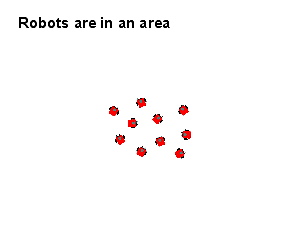
\includegraphics[width=\linewidth]{../ui_experiment/slide_images/Swarm_Robot_Control_-_Unknown_Number_of_Robots_0001.png}
	\end{subfigure}
	\begin{subfigure}{0.3\textwidth}
		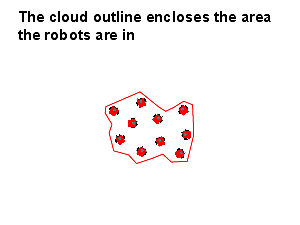
\includegraphics[width=\linewidth]{../ui_experiment/slide_images/Swarm_Robot_Control_-_Unknown_Number_of_Robots_0002.png}
	\end{subfigure}
	\begin{subfigure}{0.3\textwidth}
		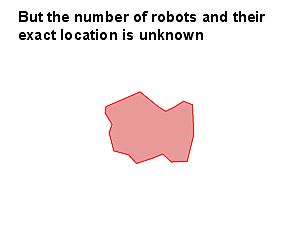
\includegraphics[width=\linewidth]{../ui_experiment/slide_images/Swarm_Robot_Control_-_Unknown_Number_of_Robots_0003.png}
	\end{subfigure}
	\caption{Instructional slides for the unknown number of robots condition, showing cloud representation of robot swarm.}
	\label{instructional_slides}
\end{figure}

\subsubsection{Selection Strategy} \label{section:Selection_Strategy}

At the end of the experiment, users were shown an image of a robot swarm, with a dotted line around it depicting a finger drag path around some of the robots. 
The users were told that the intent of this gesture was to select robots, and asked to indicate which robots in the image were selected, or in the unknown number of robots case, whether the gesture selected all of the robots or left any out. 
Users in the single robot case were shown the selection image with ten robots in it, because the with one robot, there are not enough robots to have a selection which may exclude some robots and include others. 

\begin{figure}
	\centering
	\begin{subfigure}{0.48\textwidth}
		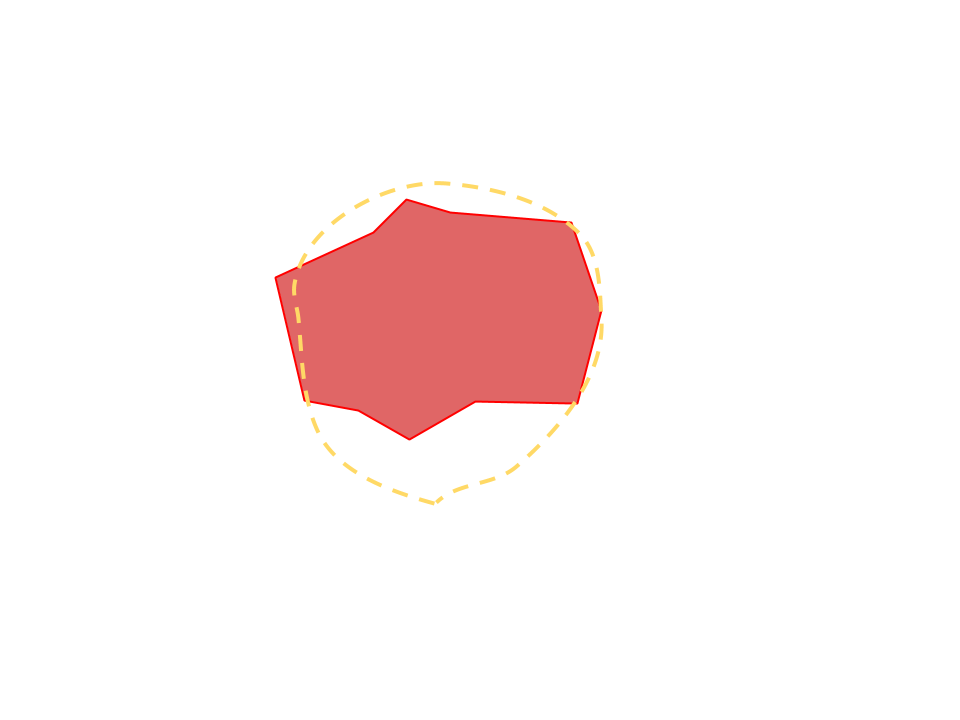
\includegraphics[width=\linewidth]{../Selection_Fuzz_X.png}
	\end{subfigure}
	\begin{subfigure}{0.48\textwidth}
		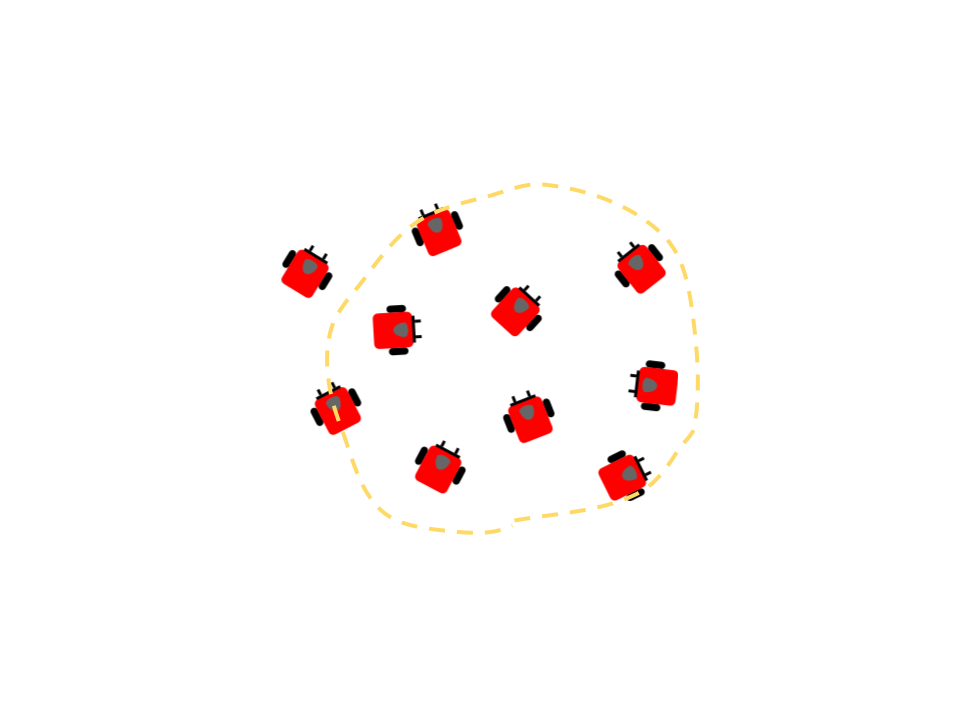
\includegraphics[width=\linewidth]{../Selection_Fuzz_10.png}
	\end{subfigure}
	\begin{subfigure}{0.48\textwidth}
		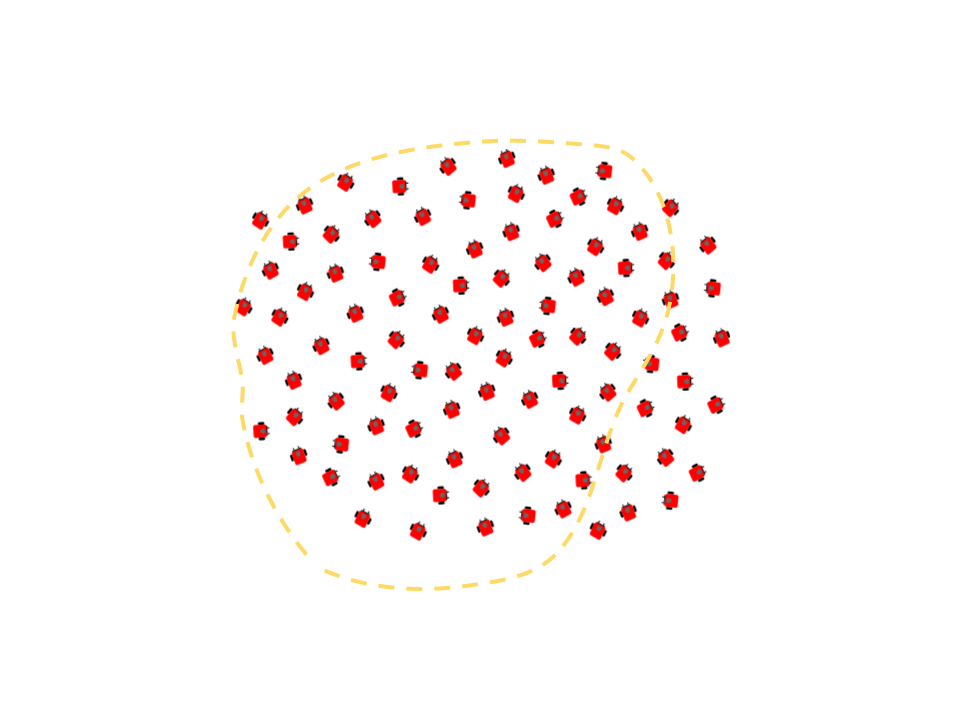
\includegraphics[width=\linewidth]{../Selection_Fuzz_100.png}
	\end{subfigure}
 	\begin{subfigure}{0.48\textwidth}
		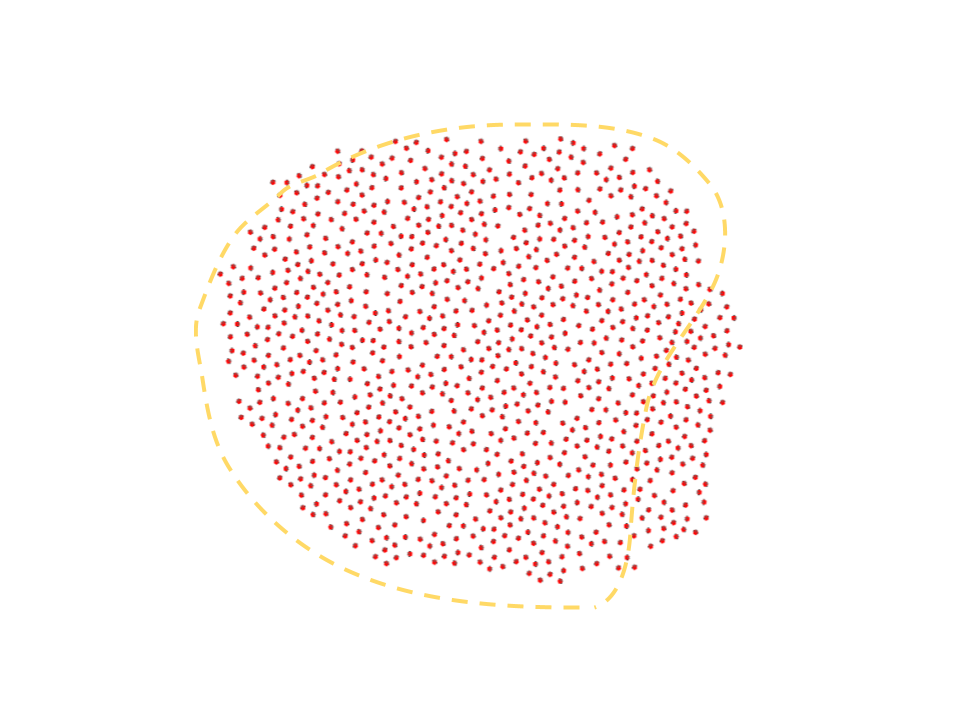
\includegraphics[width=\linewidth]{../Selection_Fuzz_1000.png}
	\end{subfigure}
		\caption{Images for selection strategy question.}
	\label{strategy_question}
\end{figure}

In the unknown number of robots case, 7 participants indicated that all the robots were selected, 3 of the participants indicated that some robots were left out, and one participant indicated that whether the selection included all of the robots could depend on the task. 

Because the 1 and 10 robot cases saw the same selection image, they are reported together. 
12 participants indicated that robots that were inside the selection or touched by the selection line should be considered selected. 
2 participants indicated that robots depicted with half or more of the robot inside the circle should be considered selected. 
One participant indicated that the robot half out of the circle should \emph{not} be selected. 
One participant indicated that robots on the border should be included or not included in the selection, depending on the task. \todo{Three answers are missing, find those and fix}
One user indicated that only the first robot touched should be selected, which is consistent with control strategies that move each robot individually. 

For the hundred robot case, 3 participants indicated that robots inside or touching the line were selected. 
3 participants said that robots should be mostly inside the line to be counted, with one participant stating that robots should be 80\% or more inside the line to count. 
2 participants indicated that robots should be more than halfway inside the line to be selected. 
One participant stated that only robots completely inside the line should be counted. \todo{One answer missing, find and fix}
 
In the thousand robot case, 7 participants indicated that robots inside or touching the line should be selected. 
2 participants indicated that robots must be completely inside the line to be selected. 
1 participant indicated that robots mostly inside the line should be selected. 

Overall, participants generally err on the side of inclusion, rather than exclusion of robots from selection.
If a user interface is required to include or exclude ambiguous elements from a selection, it appears that including ambiguous elements will satisfy users. 
User comments also suggested that ways to amend selections before further commanding the robots would be desirable.

 \begin{tabular}{ l l l l l}
   Condition & Completely inside & Half or more in & Touching line & Other\\
   \hline
   10 & 0 & 2 & 12 & 3 \\
   
   100 & 1 & 5 & 3 & 0 \\
   1000 & 2 & 1 & 7 & 0\\
   \hline
   Totals & 3 & 8 & 22 & 2 \\
 \end{tabular}

It is interesting to note that two participants, one from the unknown number of robots case, and one from the 10 robot case, said that in cases of ambiguous selection, the system should add or remove robots from the selection based on the task. 
As the system cannot predict the task it is about to be commanded to perform, it is likely best to err on the side of selecting too many robots, rather than too few. 

\subsubsection{Participant Demographics} \label{section:Participant_Demographics}

The experiment had 50 participants, 10 in each condition. 28 of the participants were male, 22 were female. The average age of participants was 22.1 years, with a standard deviation of 3.16. 

These demographics are representative of the location that the study was performed, the campus of an American college. 
It has been suggested that research in psychology focuses too much on a population that is WEIRD (Western, Educated, Industrialized, Rich, and Democratic), and that the results of such studies may not generalize beyond that population \citep{arnett2008neglected}.
However, for the purposes of this study, particularly assessing the influence of smartphone use on expectations of user interface gestures, it is useful to have a population with significant experience using smartphones, which are a product of both rich and industrialized societies. 
It is not proposed that the results of this work generalize to humanity as a whole.  

\subsection{Conclusions} \label{section:Conclusions}

In future, it would be interesting to repeat this work with a condition that does not display the robots in the user interface at all. 
We expect that for conditions such as the ``move the crate'' tasks, the user would simply indicate the crate should move to area A, without concern for which robots perform the moving. 
However, such an interface would not afford indicating particular robots or groups, so tasks such as dividing the robots around an obstacle may become impossible to perform.

During this experiment, there were some cases where the users expectations of what was possible in the interface indicated a sort of ``metaphor failure" in the user interface. 
Natural User Interfaces, of which multitouch screens are an example, are supposed to be able to leverage users' understanding of the physical world, and how objects behave in it, to build affordances for objects on the screen. 
For example, a volume knob can be displayed as an actual knob, and the screen can react appropriately to attempts to rotate the knob. 
However, people know that the objects on the screen are not e.g. knobs, switches, and so on, but pictures of those things, drawn by the computer. 
As a result, the affordances are mixed. 
The knob may afford turning, but it also affords dragging around the screen or deletion, which a knob on a real radio does not afford. 
In this study, users were tasked with stopping the robots, which had begun to move around a wall to a target area. 
One user dragged the wall in front of the robots, and another user asked if they could move the wall. 
The wall was intended to represent an actual wall, which doesn't afford moving in the physical world, but it was represented in the experiment as a thick black line. 
It may be that the users would have not attempted to move the wall if it was more clearly represented as e.g. a stone or brick wall, and so had connotations of excessive weight. 
On the other hand, the users may have regarded it as what it actually was, an image of a wall on a computer screen, and decided that since images can be moved around the screen, the wall image can too. 
Attempting to experimentally determine if the representation affects how the user interacts with the wall may require a large number of users, as out of 50 participants, only 2 even mentioned the idea of moving the wall. 

In this experiment, some users were initially confused by the interface not responding. 
It may be that running this experiment on a computer, rather than a paper prototype, contributed to the user expectation that the system could react. 
Most users' experience with touch screens is that when they touch them, something visible happens nearly immediately. 
A system that does not visibly react, as in this experiment, is usually assumed to be broken, or waiting for further input, but no one expects printed documents to react to touch.
For future work, it may be desirable to structure attempts to elicit user gestures as in Wobbrock \emph{et al.}. 
The experiment described in this section showed the initial situation, and asked the users how they would make a specific change. 
Wobbrock \emph{et al.} showed the change occurring, and then asked the users what command they would issue to cause that result. 
Showing the response before asking for the gesture removes the expectation that the system will react. 

Unfortunately, showing the response of the system may also act as a cue to the user that suggests a specific solution for gesture selection. 
For example, if the system shows a square formation being formed by multiple robots moving directly to the closest point on the square to their starting location, the paths shown are multiple direct motions. 
If instead, the system shows the robots forming a chain that snakes around the perimeter of the square before coming to a stop, the path shown is forming the snake, and then traversing the perimeter. 
The motion in the first case may suggest that the user make individual gestures to position each robot, while the gesture suggested in the second case might be more like dragging a lasso around the group and then a line from the group around the perimeter of the box. 
Even simple cases like moving to a target area, if they show the robots moving along a path, might discourage the user from using waypoints instead of dragging a path.



\chapter{Selection of Gestures for Control of Swarms}

\begin{figure}
	\centering
	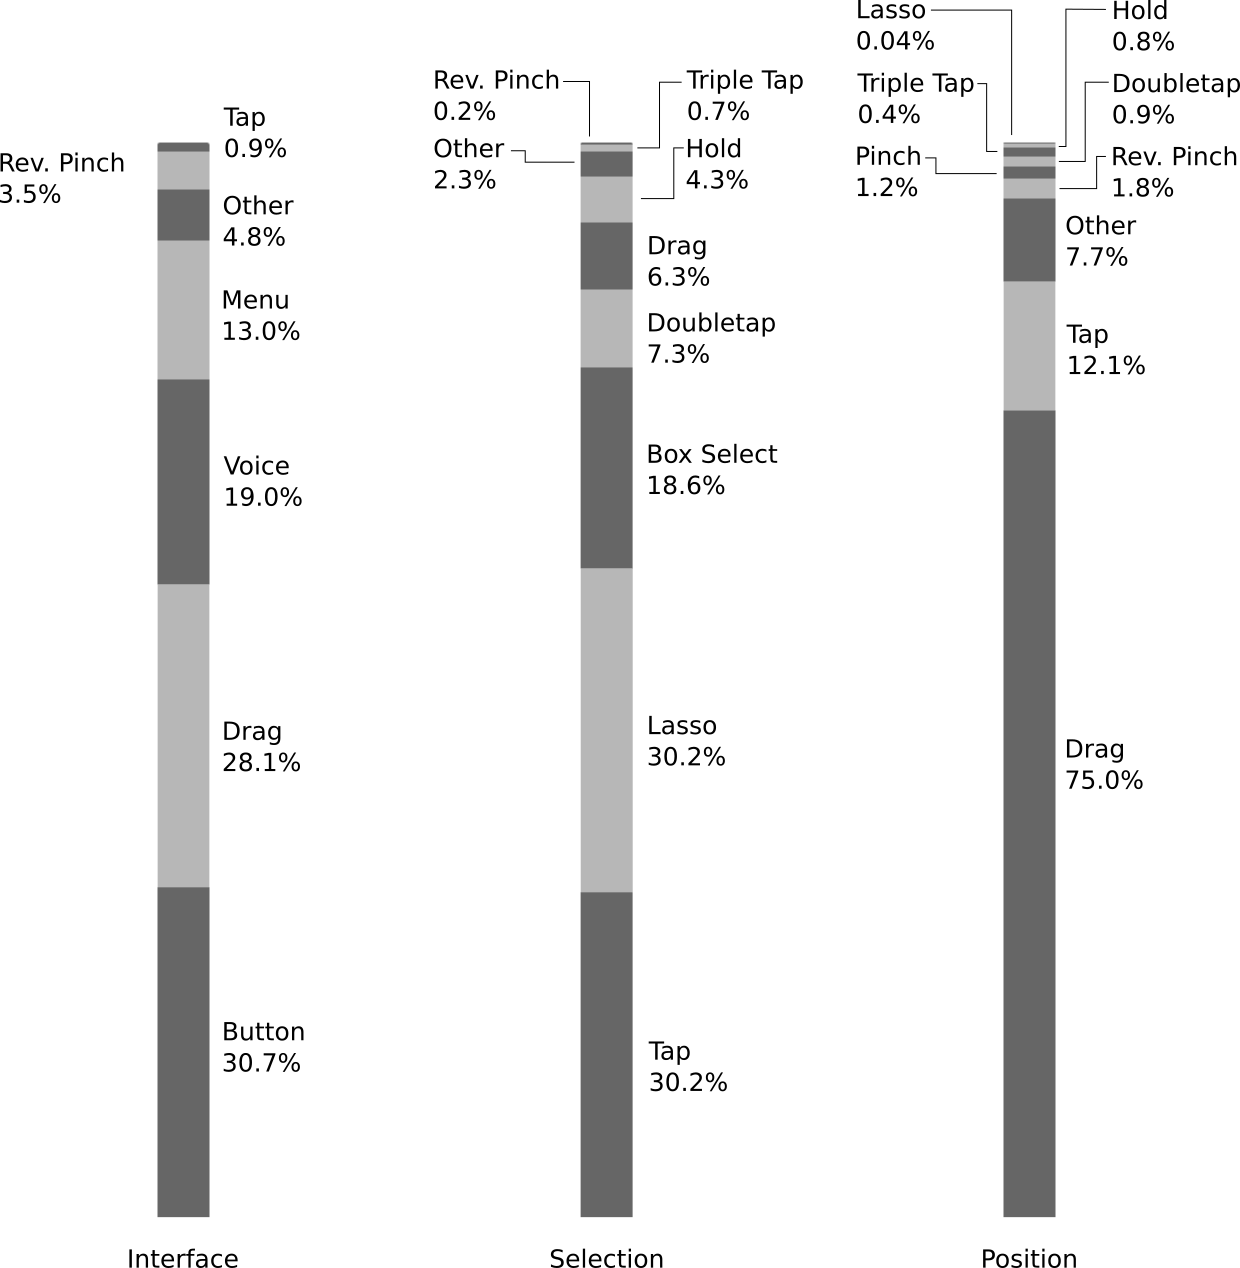
\includegraphics[width=\linewidth]{../thin_grey_text.png}
%	\begin{subfigure}{0.28\textwidth}
%		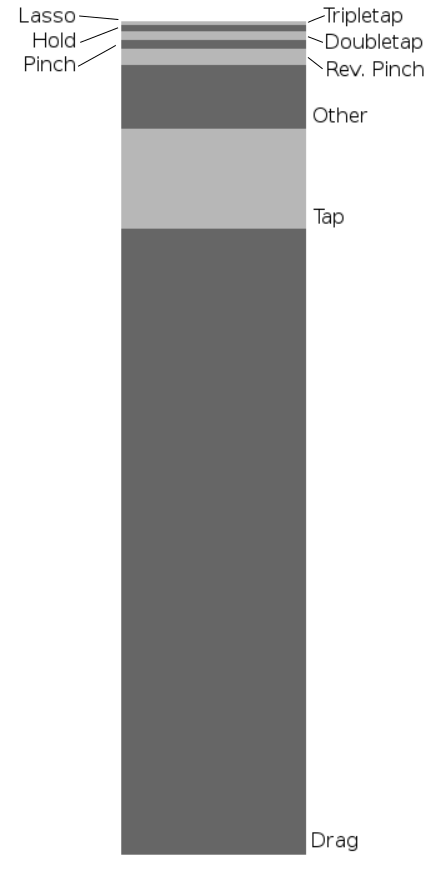
\includegraphics[width=\linewidth]{../move_grey_no_grid_text.png}
%	\end{subfigure}
%	\begin{subfigure}{0.28\textwidth}
%		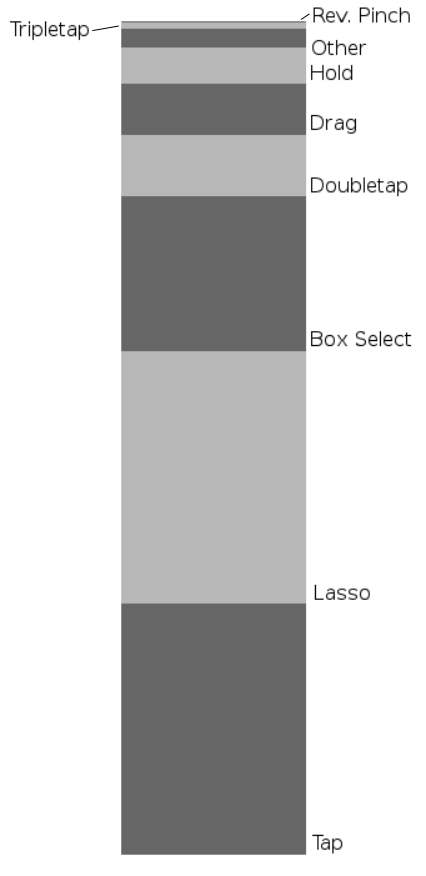
\includegraphics[width=\linewidth]{../select_grey_no_grid_text.png}
%	\end{subfigure}
%	\begin{subfigure}{0.28\textwidth}
%		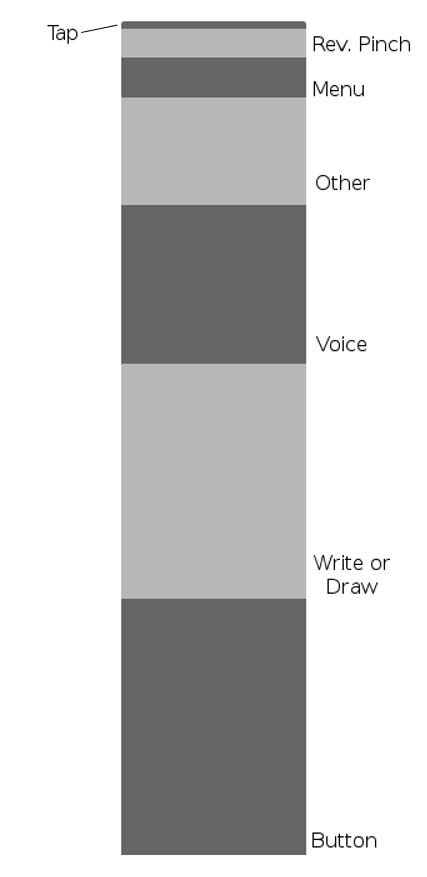
\includegraphics[width=\linewidth]{../ui_grey_no_grid_text.png}
%	\end{subfigure}
	\caption{Motion, selection, and UI gestures.}
	\label{fig:select_ui_move_breakdown}
\end{figure}


For position commands, drag, tap, and ``other'' would cover 94.8\% of the gestures. 
Unfortunately, the ``other'' commands are not a single gesture, but include a diverse collection of gestures, such as pushing with the side of the finger or making a picking-up, carrying, and setting-down motion over the screen.
As a consequence, attempting to implement all the gestures in the ``other'' category would add significant complexity to the gesture recognition in order to support gestures which were rarely used. 
Many of the ``other'' gestures were also not recognizable by a multitouch surface, such as the user dividing the robots by parting their hands as if opening a bag in the air above the surface. 
Since it does not contact the multitouch surface, such a gesture cannot be recognized without additional hardware. 
If all forms of tap are considered the same when used as position commands, taps make up 14.2\% of the position commands, and together with drag, cover 89.2\% of the position commands. 

Lasso was used as a position command by one user, who used it to command the robots to disperse in the ``disperse'' task. 
The user noted that the direction of the lasso disambiguated it from lasso as selection, so lassoing clockwise would select robots and lassoing counterclockwise would disperse them. 

Achieving 90\% recognition of the most common UI widgets would include buttons for special functions, handwriting recognition, voice commands, and other menus on the screen (totaling 90.8\%). 
However, a successful menu-based UI would not be composed simply by taking the sum of all of the user interface designs suggested by users, as there would be significant redundancy in the UI commands, and in ways of bringing up the UI for interaction. 
Instead, the tasks in which the users invoked the UI most often were examined, and the requested UI functions were considered for inclusion. \todo{Do this, figure out what they are}

Both voice commands and handwritten commands together account for 47.1\% of the user interface elements used.
While the broad categories make up nearly half of the UI elements, the individual uses of the gestures did not display a significant unity within the broad categories.
One user used symbols drawn over the swarm as commands, so a circle drawn within the swarm area meant "patrol", and would be followed by an indication of the area to be patrolled. 
Another user wrote commands, such as writing out ``0.5" to indicate that robots should divide in half, ``SQ'' to indicate that they should form a square, or ``C $\rightarrow$ A" to indicate that the crate (C) should be moved to area A. 
The majority of the drawn commands were attributable to a single user, but two users drew an `X' over the defective robot in the ``mark defective robot'' and ``remove defective robot'' tasks and two users used an `X' and an `S' in the ``stop the robots'' task.

The selection of a set of handwritten commands that would be usable for a majority of users would be a task at least as difficult as finding a user-defined set of gestures.
In addition to the set of English letters, the interface would have to consider symbols such as arrows, and apparently decimal numbers as well. 
The experiment described in this thesis did not collect sufficient examples of handwritten commands to extrapolate a useful control scheme from them.
Because of this lack of information, and the fact that most handwritten commands were proposed by a single user, the resulting interface does not contain support for handwriting recognition and symbol interpretation.  

Interestingly, voice commands were similar to both handwriting, in terms of user choice, and gestures, in terms of syntax. 
One user used voice commands for all tasks, but a few users also used voice commands for a few tasks, but not all of them. 
This distribution is like the handwritten commands, in that one user used handwritten commands frequently, but a few other users used a few of them for some tasks.
The accidental biasing of users towards use of voice for formation tasks was discussed earlier. 
In addition, two users stated that they would like to have a vocal stop command for the ``stop the robots'' task, because it could be issued quickly and without having to accurately touch the moving robots. 
These users did not issue other voice commands, as the other tasks were not perceived to be as urgent as the ``stop the robots'' task. 
The syntactic similarity between the voice commands and the gesture commands is because the gesture commands frequently take the subject-verb-object ordering of spoken sentences. 
For example, selecting the robot group indicates a subject, and drawing the path indicates the verb (``go this way"). 
Objects are optional or implied, as going to a location doesn't have a clear object that the robots are instructed to act upon. 
In some cases, the subject is implied as well.
For example, some users would make gestures intended to move the robot group as a whole by simply dragging the path, without selecting the subject first. 
In such a case, the implied subject was all of the robots. 
This sort of implication is more complex than simply assuming that if no robot is selected, all of the robots are the subject. 
Some users divided the robots into two groups by drawing a dividing line, and then dragging two paths, one to one side of the screen and the other to the other side of the screen. 
In this case, the implied subject was the half of the robots on the same side of the dividing line as the drag, but no selection gesture preceded the positioning drag to indicate this. 

%The idea of having a hidden menu that was dragged in from an edge of the screen or came up after some form of invocation, such as tap-and-hold, was rejected because such menus do not admit exploration. \todo{cite something on explorability/discovery of menus}

Reverse pinch was used as an interface command to zoom in or out of the view of the robots. This was done in the ``mark defective robot'' and ``remove defective robot'' tasks. 
The user who made this gesture was in the 1000 robot case, and stated that they wanted to zoom in because the defective robot was a small target and close to other robots. 
There was no explicit zoom or change of viewpoint task, but users expected the functionality when they had to interact with a small target.

To accommodate 90\% of the user gestures for selection, recognition of tap, lasso, box select, doubletap, drag, hold, and ``other'', totaling 91.9\% of the selection gestures.
As discussed above, the ``other'' category is not practical to implement. 
If, instead, all forms of tap are considered the same for purposes of selection, they comprise 42.5\% of the selection gestures, and together with lasso and box select, cover 91.3\% of the selections. 

Drag as a selection gesture refers to the user placing their finger on one robot, and then dragging it from robot to robot, adding each touched robot to the selection. 
It is ambiguous with the position drag, where the user places their finger on a robot and then drags a path for the robot to follow, although the distinction could be made by having a path that intersects multiple robots become a selection, rather than a position command. 
Unfortunately, this attempt at disambiguation would itself become a source of problems if the user attempts to move the entire swarm by placing a finger in the middle of it and dragging to a new location, as it is likely they would intersect more than one robot as their finger leaves the swarm.

\section{Ambiguities in Gesture Commands}

As discussed briefly in the previous section, some combinations of gestures selected by the users were ambiguous. 
This is to be expected, as the users did not know all the tasks in advance, and so might use a gesture in one task that they then felt was better suited to a later task.
The users might also not regard all the tasks as having to use a consistent and unambiguous representation for each gesture, or not remember all the gestures they had previously used. 
However, for automated conversion into programs, it is important that a sequence of gestures have some way to be unambiguously recognized. 

In the line formation tasks, some users selected the robots and then drew a line to indicate the location of the line formation.
If the line formation started at the same location as the robots, this gesture sequence is the same as the selection and drawing a path sequence that was frequently used to indicate that the robots should move as a group along the path. 
If the line formation started elsewhere, it could be disambiguated, because motion along a path almost always started on or near the selected robots.  

Similarly, some users divided the robots into two groups by drawing a line separating the groups.
Typically, this line started outside the group and passed through it, so it could be disambiguated from instructing the robots to move along the line.
Unfortunately, it would be difficult to separate it from drawing a line for the robots to move to in order to create a formation.
 
To command the robots into a square formation, especially in the dispersed cases, many users simply drew the square formation over the robots.
If a lasso select is also available, some distinction must be made between the lasso select and the square formation when they are both drawn over the robots, as they are both closed forms drawn over the robots.
One possible method is to look for peaks in the distance from each point on the perimeter of the gesture to the centroid of the gesture. 
A square would have four peaks, while a circle would have no obvious peaks. 
However, this sort of recognition means that a square lasso select, or an arbitrarily-shaped lasso select that happens to have four peaks, would get misinterpreted as a formation gesture, while a command to get into a circular formation would be interpreted as a lasso selection. 
It would be preferable to be able to make arbitrary formations, and arbitrarily-shaped lasso selections, and have them be disambiguated by some other method. 
One method that users proposed was to have a ``draw formation" button, which would then cause the next form that the user drew to be treated as the perimeter of the formation. 
Some users also held one finger down at the start of the formation, while tracing the perimeter with the other finger. 
This approach as the advantage of not adding UI elements, but is not easily discoverable by a user examining the UI. 

In order to patrol area A or the screen border, users frequently dragged the robots as if issuing a basic motion command. 
Some users indicated that there would have to be an additional signal to the robots to keep moving on the patrol route, once it was assigned, but there was not an agreement as to what that command should be. 
Of the users who indicated a need to convey that the swarm keep patrolling, some repeated the patrol route drag multiple times, others ended the gesture with a tap or triple tap, still others used the direction of the patrol route drag (clockwise or counterclockwise) to separate following the path once from continuously following it. 

Some users reused gestures for different purposes, such as tapping a robot to select it, but also tapping a robot to remove it.
Because 30.2\% of the selection gestures were taps, it was decided that selection, which occurs often, would be done by tapping, while removal of a robot, which is rare, would be performed by a different action. 


%Drawing a line to divide the robots into groups vs. drawing a path to follow vs. drawing a line for the robots to get in formation on.

The gestures used by the users could be divided between selection and position gestures, within which there was a great deal of agreement \todo{quantify agreement, maybe after Wobbrock's agreement}, and more complex actions, such as patrol, formations, picking up or moving objects, removing robots, and selection by color. 

For selection, if the system accepts taps (of any form), lasso, and box select, 91.3\% of the user selection gestures are covered. For position, tapping (again, of any form) to set goals or way points and dragging paths will cover 89.2\% of user position gestures.

Because the more complex tasks had higher variety of gestures that could be used to convey the user intent, as well as some users performing the more complex tasks by repeated selection and position gestures, attempting to handle this variety of gestures leads to two problems with the discoverability of the interface. 

First, since each of the gestures was chosen by a smaller number of the users, some training must be performed to inform users who would not have chosen that gesture. 
This training could be done with a ``cheat-sheet'' that users could pull up for reference, or an animated introductory tutorial sequence. 
These options are both less desirable than having the system be, in as much as it can be, self-explaining. 
They separate the training of the user from the user's interaction with the interface, rather than having the interface make clear what can be done.

Second, if a large percentage of the gestures for the more complex tasks were implemented, in order to provide high coverage of the various options that users chose to perform those tasks, there would be a large set of gestures that have very specific meanings. 
Increasing the set of gestures that the system recognizes increases the chances for ambiguities, where the same gesture was selected for multiple roles by different users, and for errors, where the system misinterprets one gesture as another. 
This interferes with discoverability, as the system may react in different ways to what the user felt were the same actions, confounding the user's ability to learn a mapping between their actions and the results that the system produces. 

As a result, the complex tasks were assigned to buttons on the user interface. 
The use of buttons is more discoverable, as the button simply says on it what it does. 
Buttons do obscure some of the camera view that forms the main part of the user interface, but this problem is not as severe as it might appear. 
The area the robots operate in is either bounded or unbounded.
If it is bounded, it either fits on the screen or does not fit on the screen, and if it is unbounded, it does not fit on the screen.
If the area the robots are in does not fit on the screen, the user likely views it by panning or zooming in and out, and so can pan or zoom so that the area covered by the buttons is not an area which they have to interact with to perform a task. 
If the area the robots are displayed on and interacted with in does fit on the screen, it can be shrunk slightly, and the buttons can be placed so they don't cover the interaction area. 
In either case, the design of the interface can accommodate a few buttons without seriously harming the user interaction, although the unchecked proliferation of buttons could lead to design difficulties. 